%% LyX 2.1.4 created this file.  For more info, see http://www.lyx.org/.
%% Do not edit unless you really know what you are doing.
\documentclass[english]{article}
\usepackage[T1]{fontenc}
\usepackage[utf8]{inputenc}
\usepackage{array}
\usepackage{graphicx}

\makeatletter

%%%%%%%%%%%%%%%%%%%%%%%%%%%%%% LyX specific LaTeX commands.
%% Because html converters don't know tabularnewline
\providecommand{\tabularnewline}{\\}

%%%%%%%%%%%%%%%%%%%%%%%%%%%%%% User specified LaTeX commands.
\usepackage{array}




\providecommand{\tabularnewline}{\\}

\usepackage{babel}
\graphicspath{{images/}}




\usepackage{babel}

\makeatother

\usepackage{babel}
\begin{document}

\section{One }


\section{Two}


\section{Specific Requirements}

This section of the document is dedicated at giving an in-depth description
of the platform's requirements, and is to be kept as reference during
all future phases of development.


\subsection{External interfaces}

Being MyTaxiService a fully service-oriented platform, its only external
interfaces must be those reserved for the final users; there is no
need to design specific maintenance access to the back-end system
as this is already fully standardized and does not need specific functionalities
other than the usual system administration tools.

As briefly described in section \ref{sub:User-interface}, the main
principle that must guide the design of the external interfaces of
the platform is that of business identity continuity. This section
contains a set of design mock-ups that are to be kept as reference
during the development of the user interfaces.


\subsection{Functions}


\subsection{Use Cases}

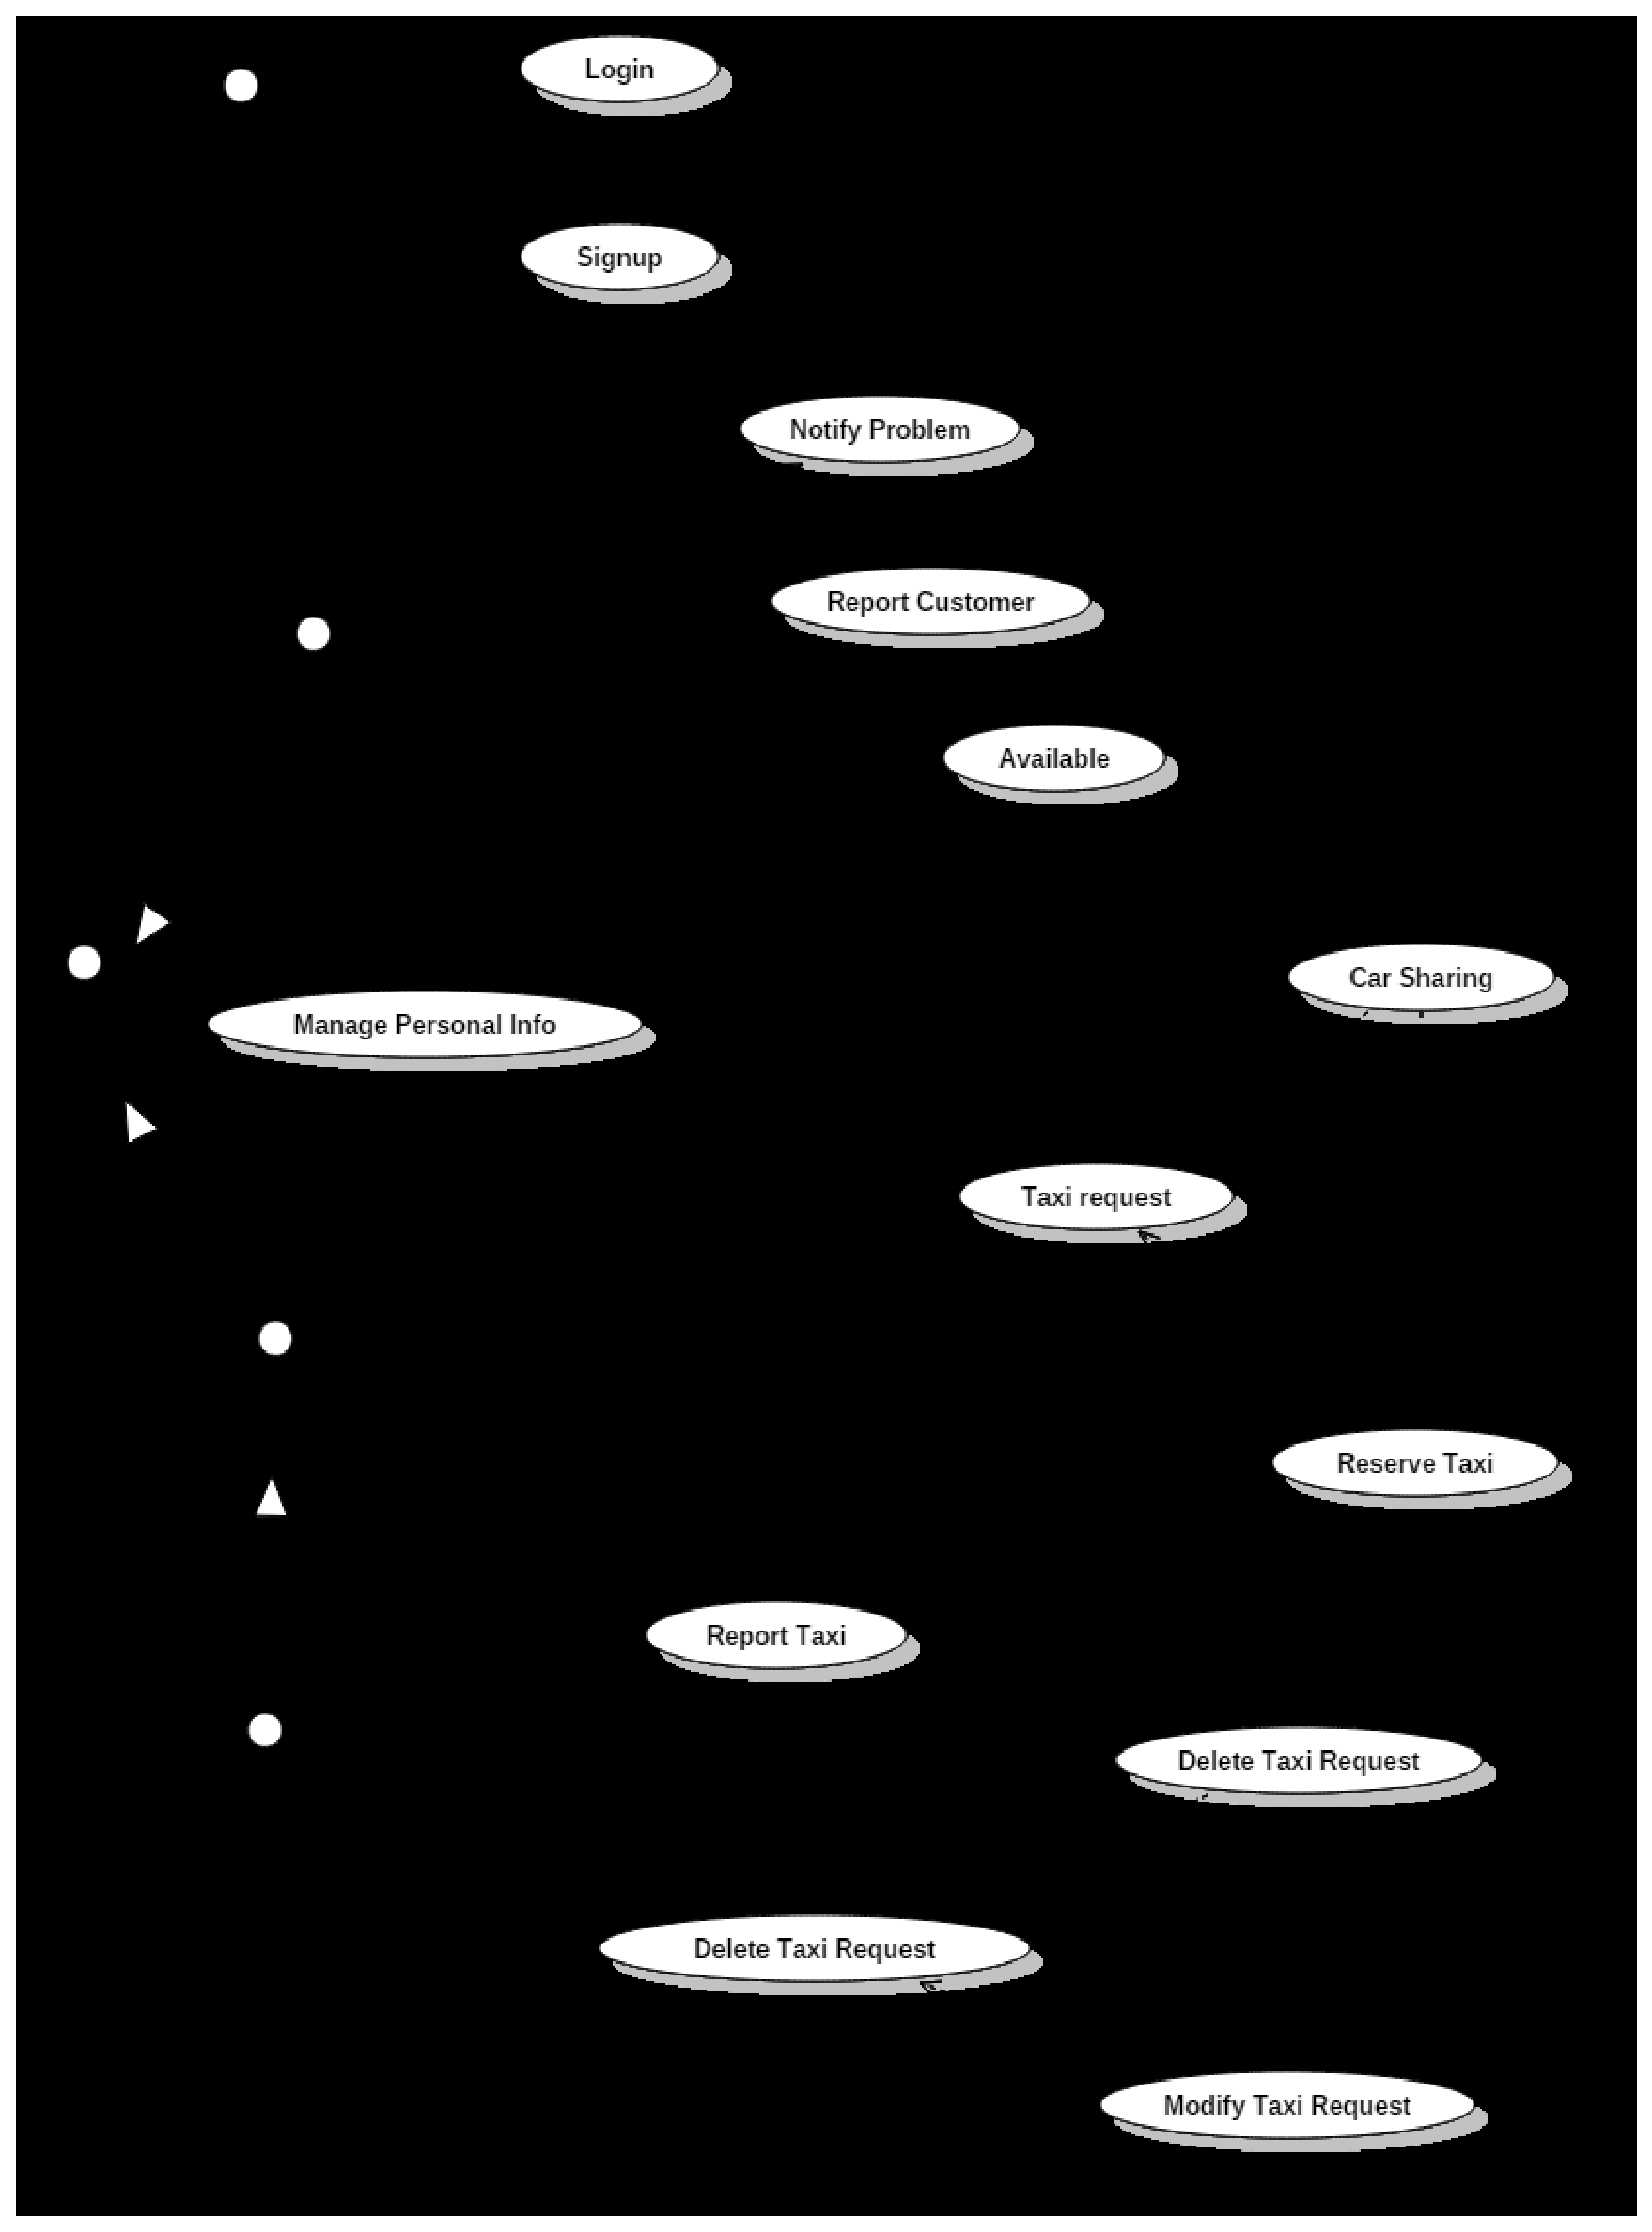
\includegraphics[width=1\textwidth]{images/png/Model1__UseCaseDiagram1_17}


\subsection{Class Diagram}

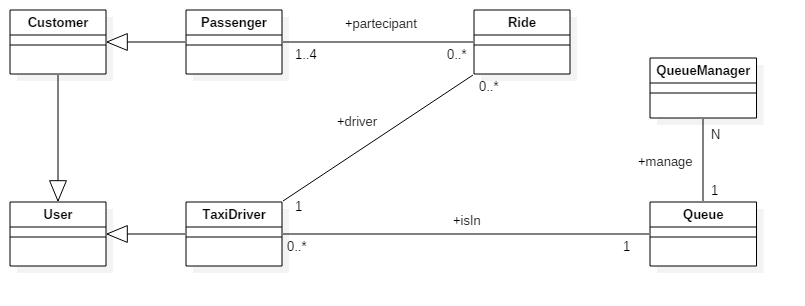
\includegraphics[width=1\textwidth]{images/png/Model2__ClassDiagram1_20}


\subsection{Scenarios}

To help the reader understand the above stated requirements, a brief
description of how a use case might look like in the real world is
given below.

In the examples, Adam, Michelle and Joanne are customers who intend
to request a taxi and Hector, Monica, Jim and Samuel are taxi drivers
of the town.


\subsubsection{Sign up}

Adam has just downloaded the customer-side app and wants to sign up
into the platform. He requests the customer registration page, fills
the form and submits the request to the system. If Adam's e-mail and
username are unique, the system gives Adam a confirmation of the success
of the operation and redirects Adam to the login page; otherwise,
an error message is displayed on Adam's phone.


\subsubsection{Login}

Adam, now registered, inserts the username and password in the login
form and clicks the login button; the system checks the information
and, if the username-password combination is correct, redirects Adam
to his own user profile page; otherwise, an error message is displayed
on Adam's phone.


\subsubsection{Available}

Hector, already logged into the platform, starts his working by day
opening his taxi-side application and communicating his availability
to the system. The system updates the taxi queue in Hector's zone
and sends Hector a notification with his position in the queue.


\subsubsection{Taxi request}

Adam, now logged into the system, wants to book a taxi to go home.
He opens the taxi request page on the app, and requests a taxi. The
system forwards Adam's request to the queue associated with Adam's
position, and Hector, which is the first taxi driver in the queue,
is notified with the request.

Unfortunately, Hector has now decided to take a break and does not
want to take charge of this ride; he refuses Adam's request by tapping
a button on the app, and the system forwards the request to Monica,
the taxi driver immediately after Hector in the queue.

As she accepts Adam's request, Adam receives a notification on the
app with the estimated waiting time.


\subsubsection{Book a Taxi}

While on Monica's taxi, Adam wants to book a taxi for that evening
at 6 PM, in order to go to the cinema. He opens the \textit{Taxi request}
page of the app, and fills and submits the request form.

The system checks the information (sending eventual error notifications
back to Adam) and forwards Adam's request to Jim, by using a specific
selection algorithm over taxi drivers in the queue associated to Adam's
zone.

Jim decides to accept Adam's booking, and will keep his schedule free
for the time that Adam requested.


\subsubsection{Car sharing}

Michelle and Joanne live in the same neighborhood, and they both decide
to go see a fair on the other side of the Town. Since they are both
short on money, after opening the \textit{Taxi request }page of the
app they both check the \textit{car sharing }option; they then submit
their requests. 

The system performs a check on Michelle and Joanne's requests


\subsubsection{Manage \textit{Reserve Taxi} Request}

Later that day, Adam browses the platform's website from his laptop's
browser, and opens the \textit{Manage taxi request} page to change
the booking time from 6PM to 7PM. 

The system checks whether Adam's request is acceptable (there must
be at least two hours between the current time and the requested time),
and eventually forwards the changes to Jim.

Jim accepts the modification and a confirmation is sent back to Adam.


\subsubsection{Report Taxi}

Jim picks Adam up at 7PM. During the ride Jim lights up a cigarette
and is unreasonably rude towards Adam.

Adam opens the \textit{Report taxi} page on the app, to file a complaint
about Jim's behavior. The system updates Jim's profile information
with the new report and confirms the success of the operation to Adam.


\subsubsection{Report Customer}

After the ride, Adam is annoyed by the behavior of Jim and refuses
to pay for the ride.

Jim opens the \textit{Report user} page, fills the complaint form
and submits it to the system. The system updates Adam's profile information
with the new report and confirms the success of the operation to Jim.


\subsubsection{Manage Personal Information}

Joanne has opened a new main email account.

She opens her profile page from the app, clicks on the \textit{edit}
button and changes her email address to match the new one; she then
submits the new information.

The system performs a check on the information, updates Joanne's profile
and notifies the success of the operation to Joanne.


\subsubsection{Report Problem}

During a ride, Hector has a problem with his taxi's engine and can't
bring Joanne to her destination.

Through the \textit{Report problem} page of the app, he notifies the
problem to the system by filling the form and submitting. The system
acknowledges the report and asks Hector if he'll be needing a new
taxi; Hector confirms, and the system forwards his request to Samuel,
who is the first taxi driver in Hector and Joanne's current zone.


\subsection{Flow of events}


\subsubsection{Sign-up}

\begin{tabular}{lp{8cm}}
\hline 
Actors  & Guest \tabularnewline
\hline 
Preconditions  & The guest is not registered into the system \tabularnewline
\hline 
Execution Flow  & \begin{enumerate}
\item The guest requests the registration page 
\item The system asks for the sign-up information 
\item The guest fills the form and submits the request 
\item The system checks the uniqueness of the username and e-mail 
\item The system creates the customer (or taxi driver) profile 
\item The system sends the confirmation to the guest \end{enumerate}
\tabularnewline
\hline 
Postconditions  & The guest is now a registered user \tabularnewline
\hline 
Exceptions  & The e-mail or username are not unique or, in the case of a taxi driver
sign-up, the license is not valid \tabularnewline
\end{tabular}

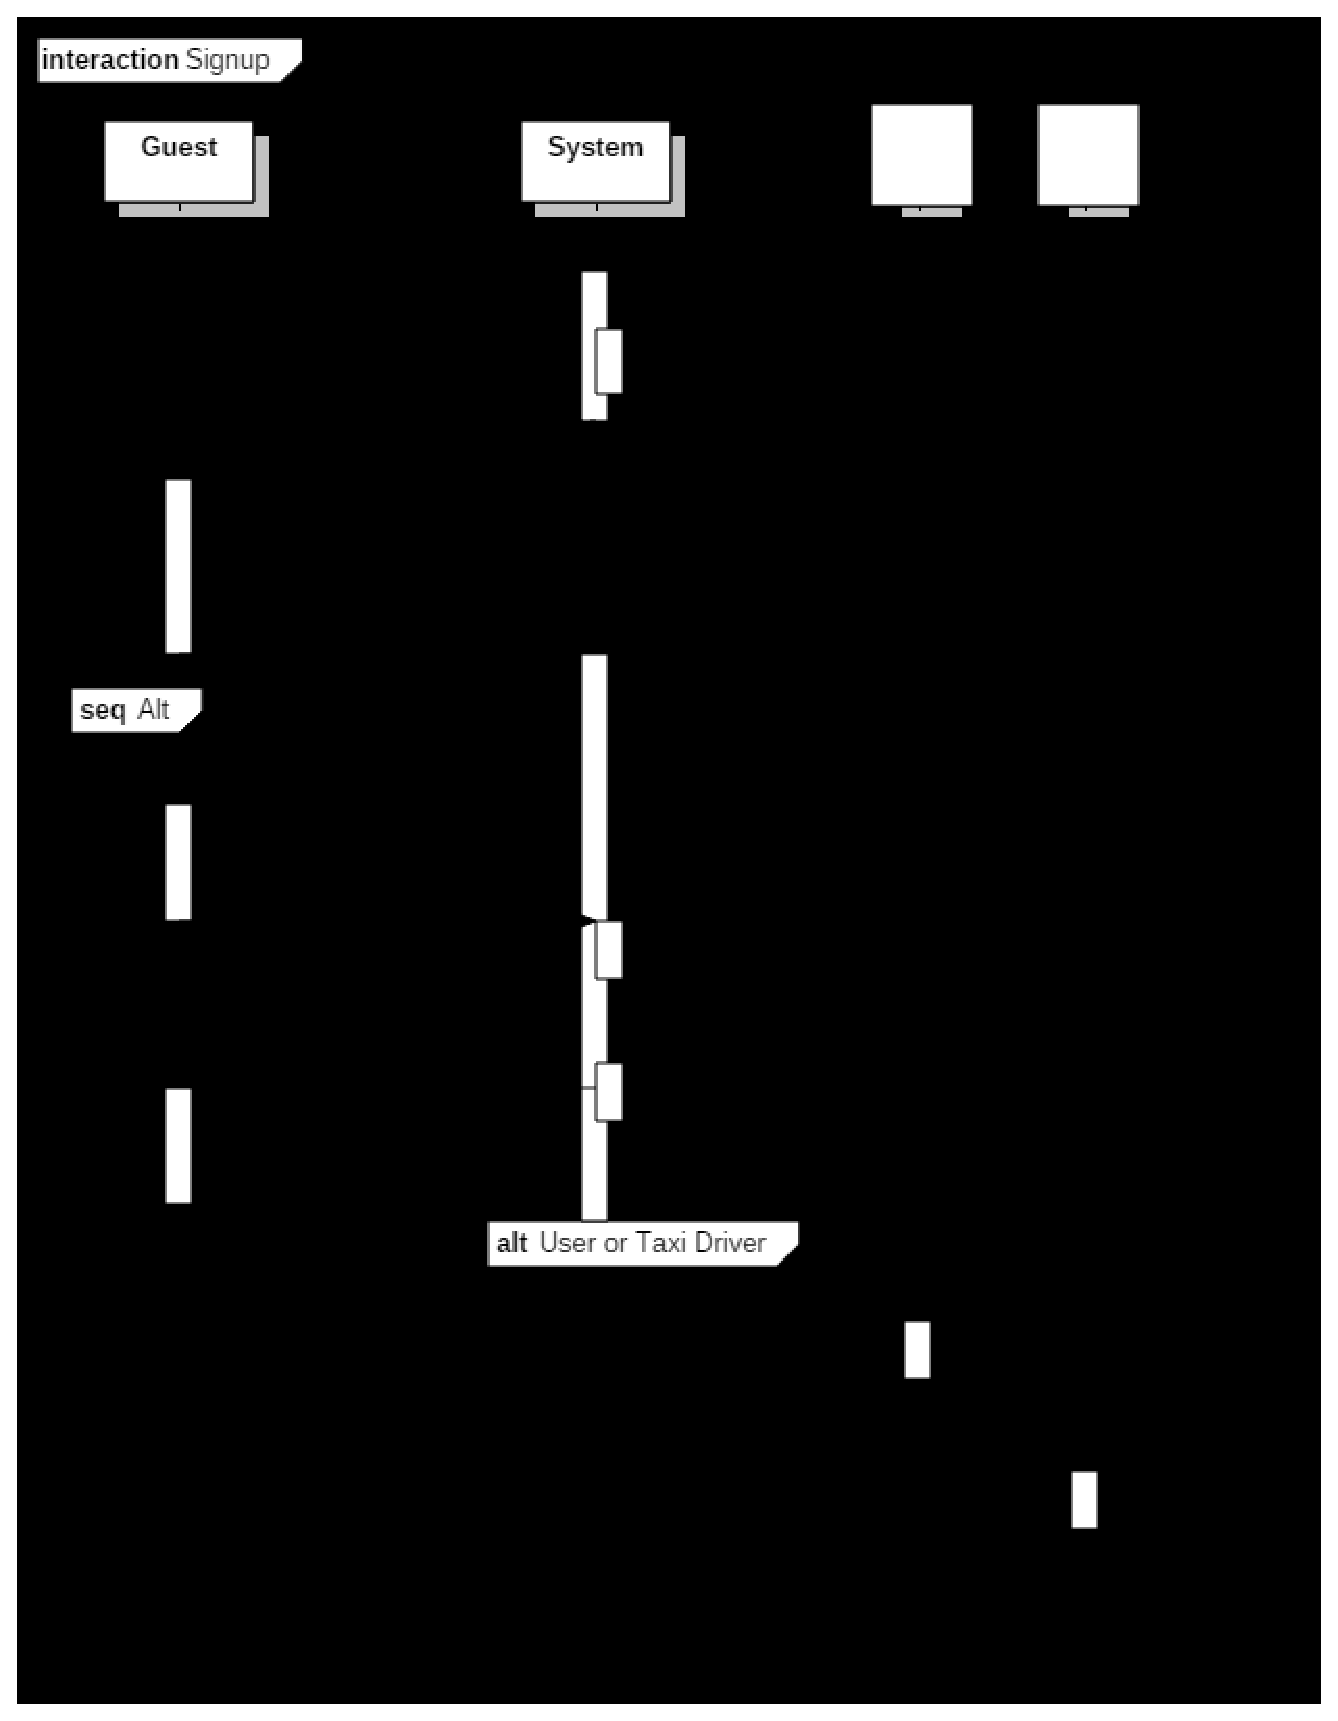
\includegraphics[width=1\textwidth]{images/png/Collaboration1__Interaction1__Signup_2}


\subsubsection{Login}

\begin{tabular}{lp{8cm}}
\hline 
Actors  & Guest \tabularnewline
\hline 
Preconditions  & The guest has already a profile into the system\tabularnewline
\hline 
Execution Flow  & \begin{enumerate}
\item The guest requests the login page 
\item The system requires the login information (Username, password) 
\item The guest fills the form and submits the request 
\item The system checks the username and password 
\item The system sends a login confirmation 
\item The guest is logged into the system 
\item The guest is redirected to the user profile page \end{enumerate}
\tabularnewline
\hline 
Postconditions  & The guest is now a logged-in user\tabularnewline
\hline 
Exceptions  & The username-password combination is incorrect, so the guest cannot
log in \tabularnewline
\end{tabular}

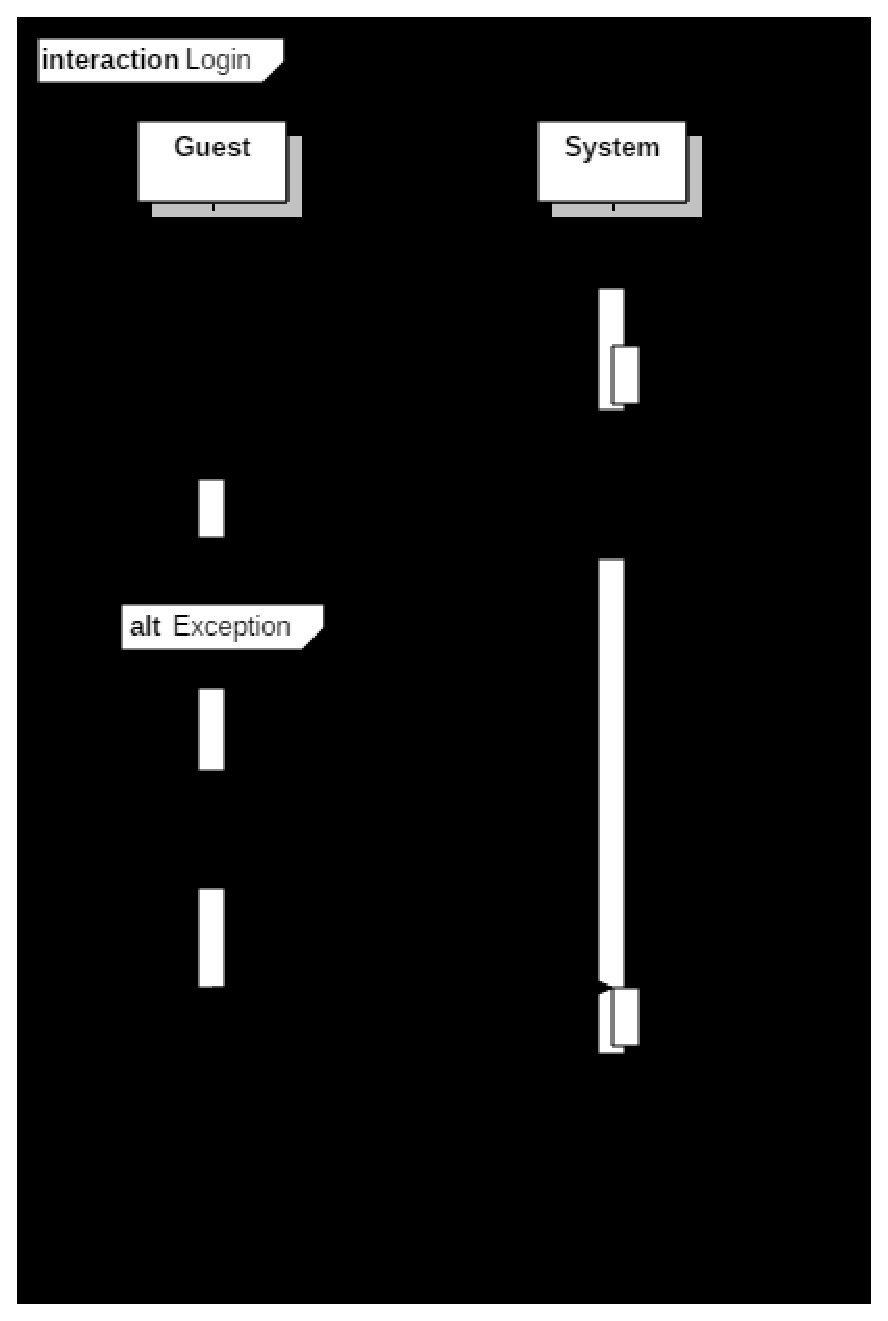
\includegraphics[width=1\textwidth]{images/png/Collaboration2__Interaction1__Login_3}


\subsubsection{Available}

\begin{tabular}{lp{8cm}}
\hline 
Actors  & Taxi driver \tabularnewline
\hline 
Preconditions  & \tabularnewline
\hline 
Execution Flow  & \begin{enumerate}
\item The taxi driver requests their profile page 
\item The system displays the user's personal information 
\item The taxi driver can choose to change their availability, becoming
available or unavailable 
\item The taxi driver sends the request to the system 
\item The system updates the queue 
\item The system returns a confirmation to the taxi driver \end{enumerate}
\tabularnewline
\hline 
Postconditions  & The taxi driver is now available \tabularnewline
\hline 
Exceptions  & \begin{itemize}
\item The taxi driver is located in a invalid zone 
\item The taxi driver is carrying a passenger 
\item The taxi driver is not available\end{itemize}
\tabularnewline
\end{tabular}

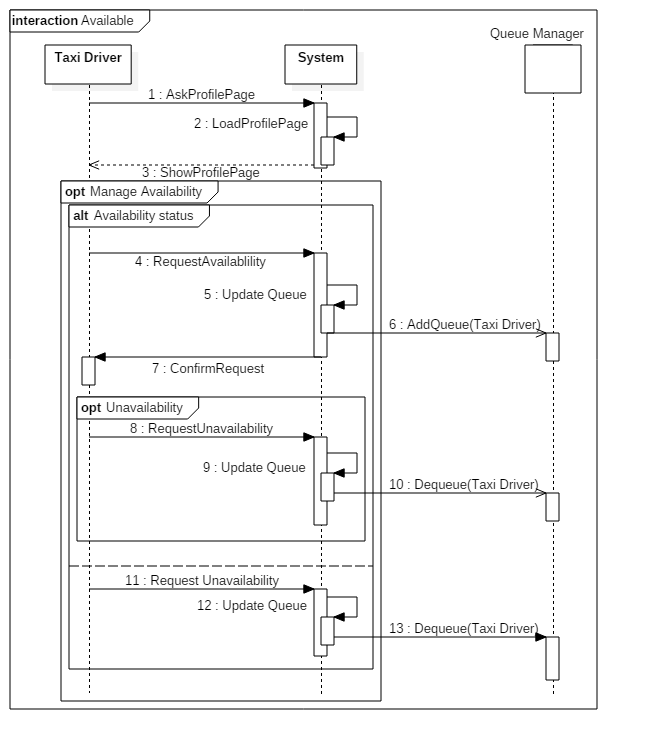
\includegraphics[width=1\textwidth]{images/png/Collaboration10__Interaction1__Available_11}


\subsubsection{Taxi Request}

\begin{tabular}{lp{8cm}}
\hline 
Actors  & Customer, Taxi driver \tabularnewline
\hline 
Preconditions  & The user should not be banned \tabularnewline
\hline 
Execution Flow  & \begin{enumerate}
\item The customer requests the \textit{Taxi request} page 
\item The system asks for the type of request that the user wants to issue 
\item The customer fills the request form and sends the information to the
system 
\item The system forwards the request to the first taxi driver of the local
queue 
\item If the taxi driver answers positively to the request, he takes charge
of the ride, otherwise he denies the request 
\item If the taxi driver accepts the request, the system notifies to the
customer the incoming taxi and changes the availability of the taxi
driver; otherwise, the system updates the queue and forwards the request
to the new first taxi driver of the queue. 
\item If there are no taxis available, the system notifies so to the user.\end{enumerate}
\tabularnewline
\hline 
Postconditions  & If the request is accepted by a taxi driver, the customer is now a
passenger \tabularnewline
\hline 
Exceptions  & \begin{itemize}
\item The customer provides incorrect information in the request form 
\item The customer is not in a valid position (\emph{e.g. outside the town}) \end{itemize}
\tabularnewline
\end{tabular}

\includegraphics[width=1\textwidth]{\string"images/png/Collaboration3__Interaction1__Taxi Request_4\string".eps}


\subsubsection{Manage \textit{Reserve Taxi} Request}

\begin{tabular}{lp{8cm}}
\hline 
Actors  & Passenger \tabularnewline
\hline 
Preconditions  & \tabularnewline
\hline 
Execution Flow  & \begin{enumerate}
\item The passenger requests the \textit{Taxi request management} page 
\item The page is generated by the system on the user's app
\item The passenger can modify the request by filling the \textit{Modify
request }form
\item The system modifies the request and returns a confirmation to the
passenger 
\item The passenger can delete the request, submitting the operation to
the system 
\item The system updates the queue and returns a confirmation to the passenger \end{enumerate}
\tabularnewline
\hline 
Postconditions  & \begin{itemize}
\item If the passenger chooses to modify the request, the request is updated 
\item If the passenger chooses to delete the request, the request is canceled\end{itemize}
\tabularnewline
\hline 
Exceptions  & \begin{itemize}
\item The passenger provides incorrect information in the \textit{Modify
request} form 
\item The passenger cancel the request too late \end{itemize}
\tabularnewline
\end{tabular}

\includegraphics[width=1\textwidth]{\string"images/png/Collaboration15__Interaction1__Manage reserve Taxi Request_19\string".eps}


\subsubsection{Report Taxi}

\begin{tabular}{lp{8cm}}
\hline 
Actors  & Passenger \tabularnewline
\hline 
Preconditions  & \tabularnewline
\hline 
Execution Flow  & \begin{enumerate}
\item The passenger requests the \textit{Report taxi} page 
\item The page is shown on the customer's application
\item The passenger fills the form and submits the report 
\item The system checks the submitted data
\item The system updates the taxi driver information 
\item The system notifies to the passenger the success of the operation \end{enumerate}
\tabularnewline
\hline 
Postconditions  & The taxi driver is reported by the passenger \tabularnewline
\hline 
Exceptions  & The passenger provides incorrect information in the report form \tabularnewline
\end{tabular}

\includegraphics[width=1\textwidth]{\string"images/png/Collaboration7__Interaction1__Report Taxi_8\string".eps}


\subsubsection{Report Customer}

\begin{tabular}{lp{8cm}}
\hline 
Actors  & Taxi driver \tabularnewline
\hline 
Preconditions  & The interaction between customer and taxi driver must have happened
at least 24 hours before\tabularnewline
\hline 
Execution Flow  & \begin{enumerate}
\item The taxi driver requests the\textit{ Report customer} page 
\item The page is shown on the taxi driver's application
\item The taxi driver fills the form and submits the report 
\item The system checks the submitted data
\item The system updates the user information 
\item The system notifies to the taxi driver the success of the operation \end{enumerate}
\tabularnewline
\hline 
Postconditions  & The customer is reported by the taxi driver \tabularnewline
\hline 
Exceptions  & The taxi driver provides incorrect information in the report form \tabularnewline
\end{tabular}

\includegraphics[width=1\textwidth]{\string"images/png/Collaboration13__Interaction1__Report Customer_14\string".eps}


\subsubsection{Manage Personal Information}

\begin{tabular}{lp{8cm}}
\hline 
Actors  & Customer or Taxi driver \tabularnewline
\hline 
Preconditions  & \tabularnewline
\hline 
Execution Flow  & \begin{enumerate}
\item The user requests the their profile page 
\item The user's personal information is shown on the user's application
\item The user can request to edit their profile 
\item The system returns the editable information of the profile 
\item The user can edit their information and send the changes to the system 
\item The system performs a check on the new information 
\item If the information is correct, a confirmation is sent back to the
user; otherwise, an error messagge is shown. \end{enumerate}
\tabularnewline
\hline 
Postconditions  & If the user modifies their profile with correct information, the profile
is changed \tabularnewline
\hline 
Exceptions  & The user provides incorrect information \tabularnewline
\end{tabular}

\includegraphics[width=1\textwidth]{\string"images/png/Collaboration9__Interaction1__Manage your Personal Info_10\string".eps}


\subsubsection{Report Problem}

\begin{tabular}{lp{8cm}}
\hline 
Actors  & Taxi driver \tabularnewline
\hline 
Preconditions  & \tabularnewline
\hline 
Execution Flow  & \begin{enumerate}
\item The taxi driver requests the \textit{Report problem} page 
\item The page is shown on the taxi driver's application
\item The taxi driver fills the form and submits the information 
\item If the taxi driver has a passenger on board, they can request another
taxi to drive the passenger to their destination
\item If the taxi driver requests another taxi the system looks for an available
taxi driver 
\item If an available taxi driver is found, a notification is sent to both
drivers. 
\item If the new taxi driver accepts the ride, a confirmation is sent to
the driver who is submitting the report; otherwise, the systems looks
for other taxi drivers until someone accepts the ride, and returns
a failure notification otherwise. \end{enumerate}
\tabularnewline
\hline 
Postconditions  & The problem is reported to the system \tabularnewline
\hline 
Exceptions  & \begin{itemize}
\item The taxi driver is located in a invalid zone 
\item The taxi driver fills the form with incorrect information\end{itemize}
\tabularnewline
\end{tabular}

\includegraphics[width=1\textwidth]{\string"images/png/Collaboration14__Interaction1__Notify Problem_18\string".eps}


\subsection{Entities Behavior}


\subsubsection{User}

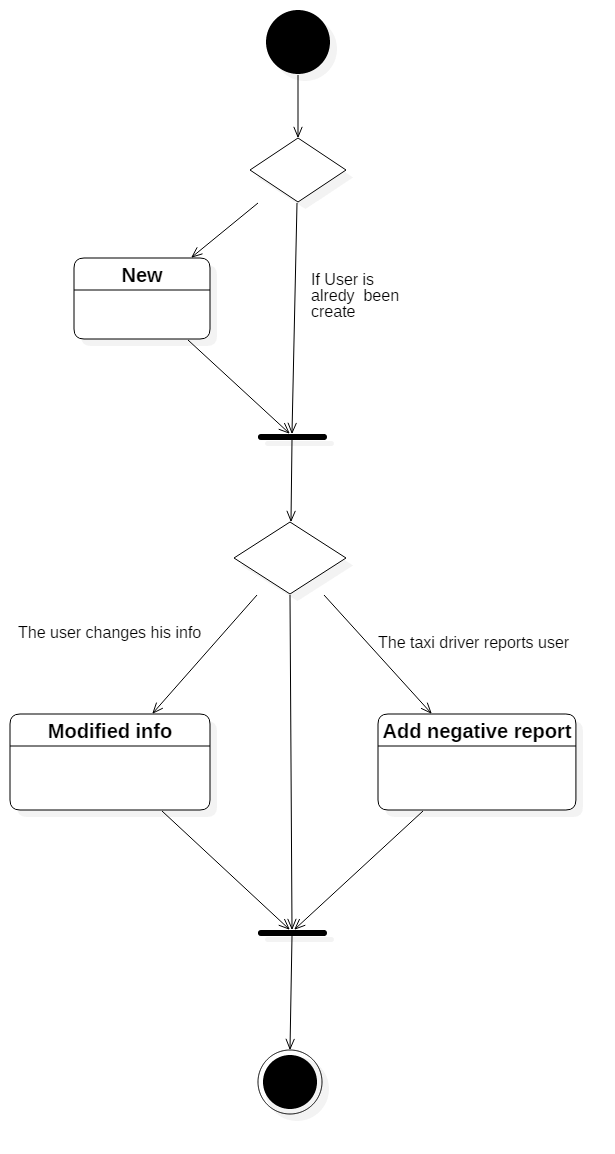
\includegraphics[width=1\textwidth,height=1\textheight]{images/png/StateMachine3__User_23}


\subsubsection{Ride}

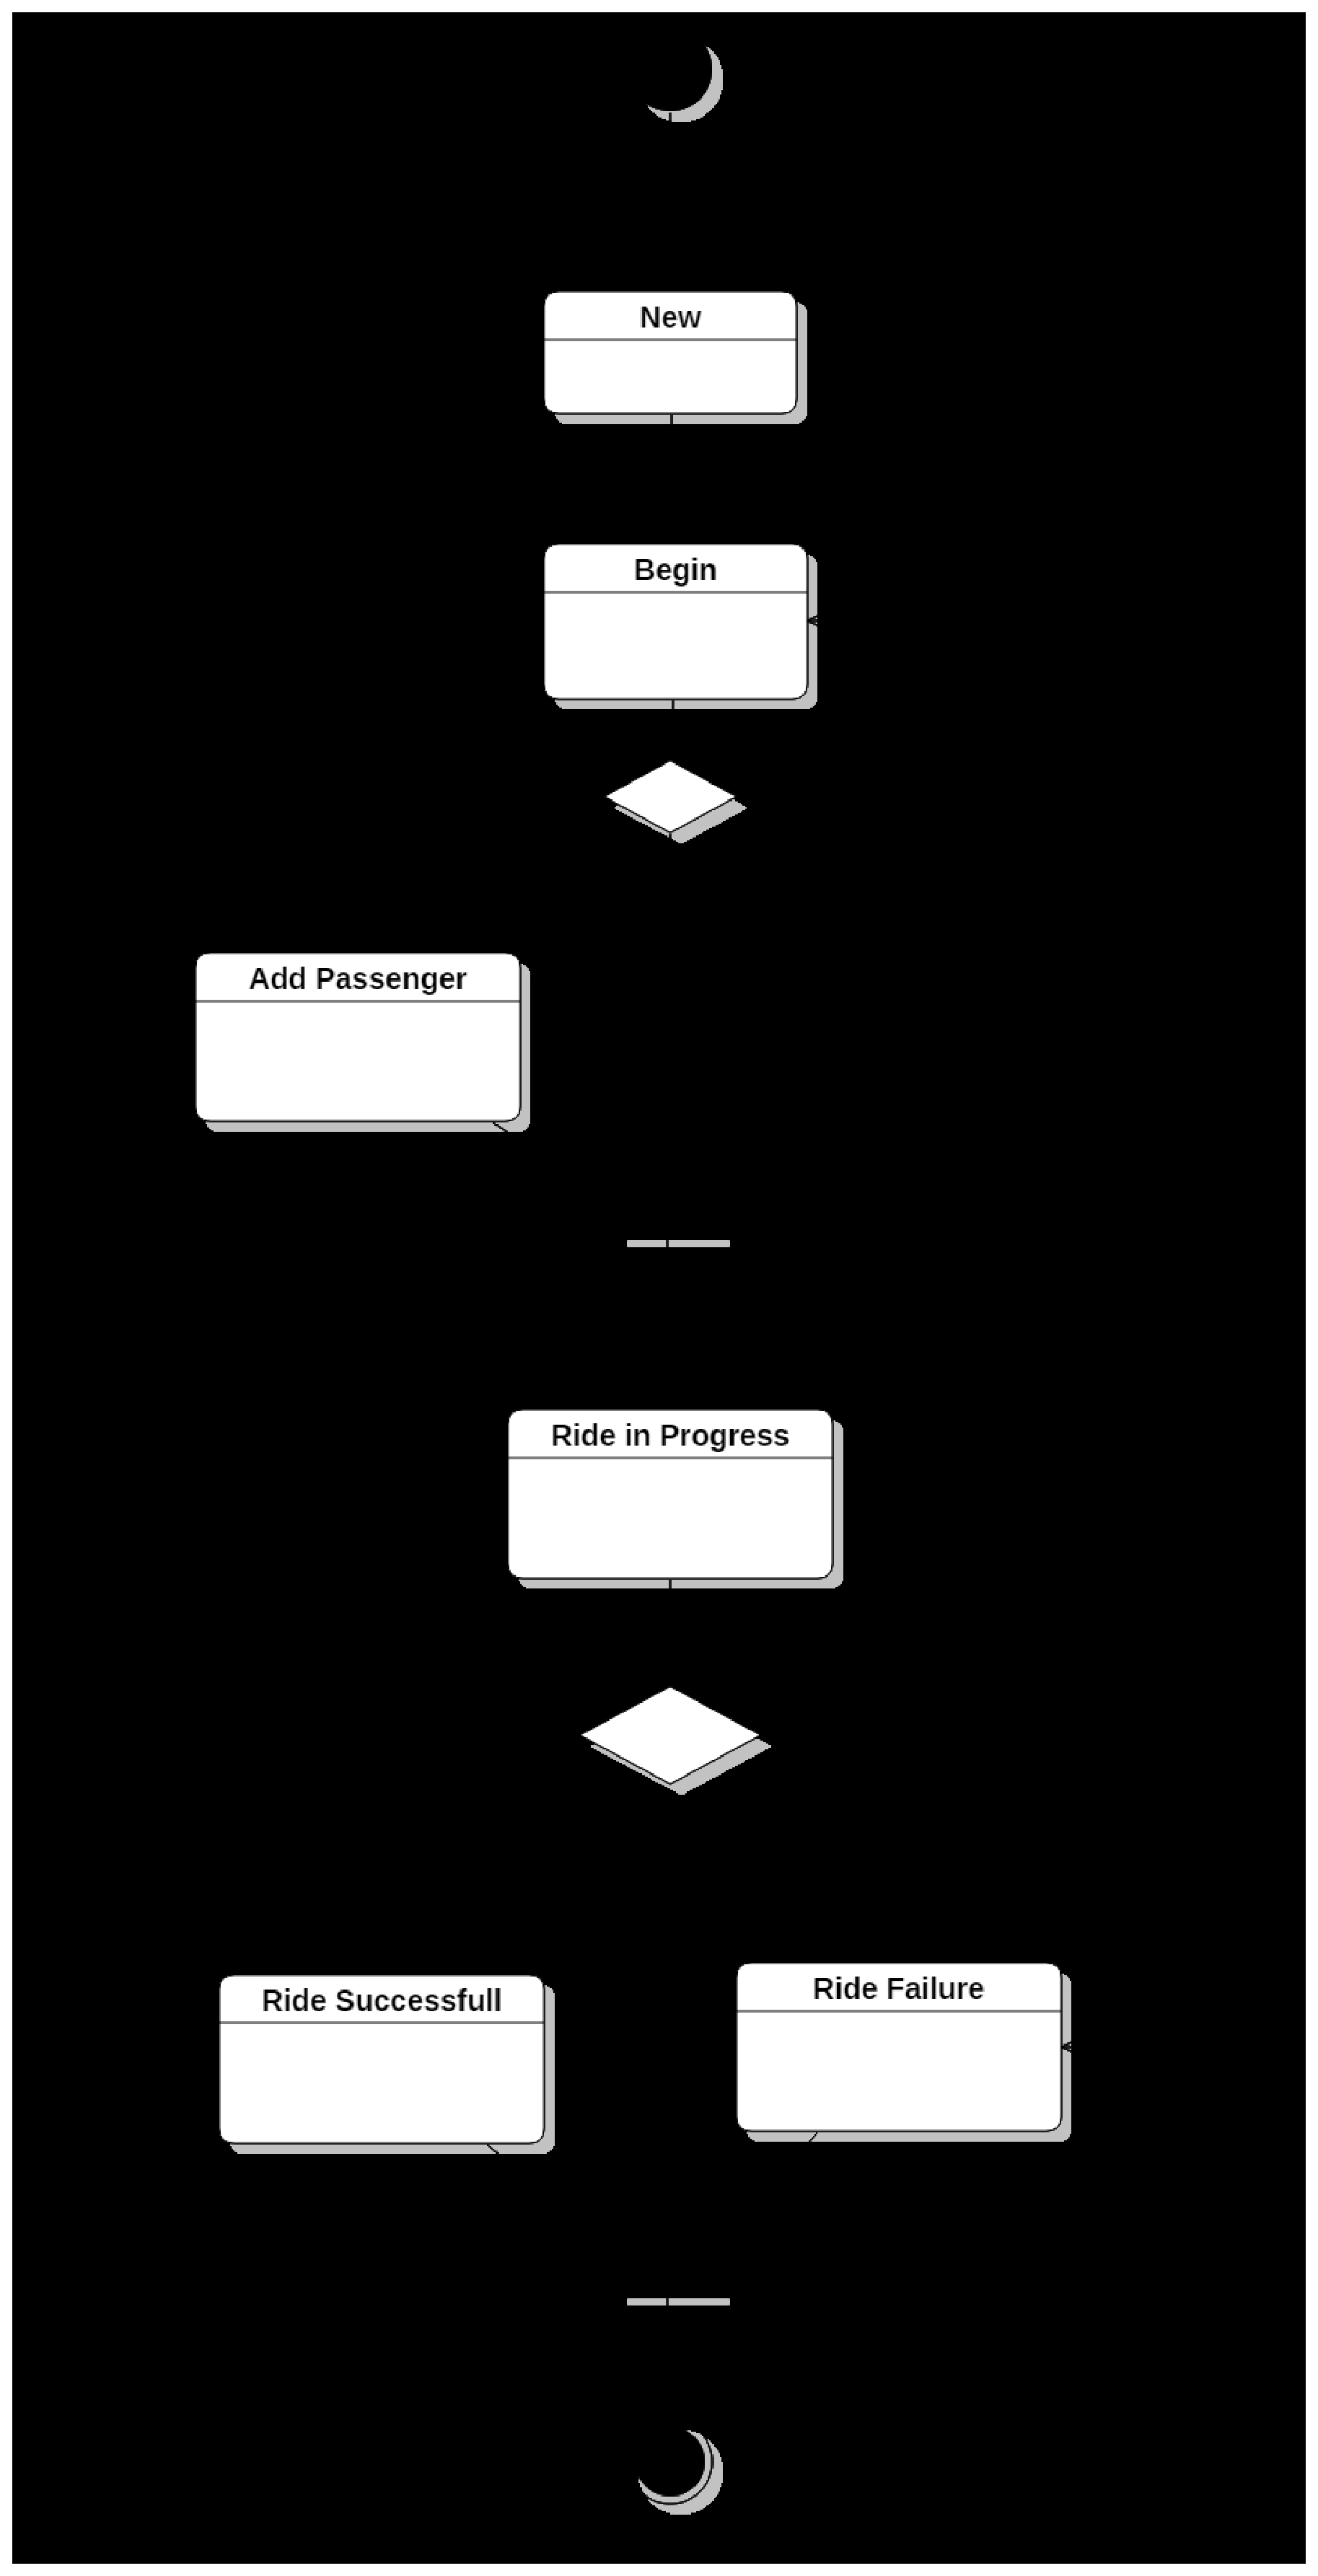
\includegraphics[width=1\textwidth,height=1\textheight]{images/png/StateMachine2__Ride_22}


\subsubsection{Queue Manager}

\includegraphics[width=1\textwidth,height=1\textheight]{\string"images/png/StateMachine1__Queue Manager _21\string".eps}


\subsection{Performance requirements}
\begin{itemize}
\item The system should support at least all the taxi driver registered
into the Town Database 
\item The system should elaborate user incoming information 
\item The system should provide the faster path for each ride 
\item The system should calculate the final price of the ride with a maximum
error of 10\% 
\item The system should provide to a passenger the arrival time (maximum
error 20\%) and change the path in case of traffic 
\end{itemize}

\subsection{Logical database requirements}
\begin{itemize}
\item The system databases has consistency check, data integrity check 
\end{itemize}

\subsection{Design constraints}
\begin{itemize}
\item GPS precision limitations: average 3m error 
\item Internet congestion 
\end{itemize}

\subsection{Standards compliance}


\subsection{Software system attributes}


\subsection{Availability and Reliability}

Since MyTaxiService is a service-oriented platform, its reliability
parameters directly relate to its availability parameters. The platform's
ability to function under the stated conditions is indeed its ability
to respond to users' requests at any given time, hence the strict
relation between the two. It has been decided to treat the two aspect
as one, and the related non functional requirements are listed in
this section.
\begin{enumerate}
\item The platform's services must be available to the users 24/7.
\item The RTO parameter must be kept at minimal levels (less than 1 minute)
at any given time.

\begin{enumerate}
\item Mission critical data must be locally mirrored on fast hardware (e.g.
stored in RAID1 arrays with flash storage).
\end{enumerate}
\item The RPO parameter must be kept at minimal levels (less than 10 seconds)
at any given time.

\begin{enumerate}
\item Any data must be locally stored in a 10 second time frame from its
creation.
\item Any locally stored data must be locally and remotely mirrored in a
1 minute time frame from its memorization. 
\end{enumerate}
\item Data integrity checks must be periodically performed between the main
data storage unit and the secondary backups, in order to ensure the
success of disaster recovery operations.
\item The implementation of the platform must prefer the absence of service
to an incorrect or unsound one. 

\begin{enumerate}
\item No data exchanges must happen during the disaster recovery operations.
\item Data stored in memory in the event of a system failure or security
breach must be considered corrupt and no attempts must be made at
recovering it. 
\end{enumerate}
\end{enumerate}

\subsection{Security}

The following non functional requirements cover the security aspects
of the platform in order, among other reasons, to satisfy the C3 constraint
in section \ref{sub:Constraints}.
\begin{enumerate}
\item Access to the user data through the intended applications must be
password protected.

\begin{enumerate}
\item A ban system must exists to prevent brute-forcing of the users' passwords.
\end{enumerate}
\item Sensitive user data (like passwords) must be stored under at least
one encryption layer, after having been \textit{salted}. This applies
to secondary storage, too. 

\begin{enumerate}
\item Decryption of the above mentioned data must happen exclusively at
runtime and the \textit{cleartext }information must never be sent
through any communication channels. 
\end{enumerate}
\item Operations on the platform must be performed exclusively by logged
users (with the exception of the guest registration).
\item HTTP data exchanges between the back-end and the user-side applications
must be encrypted with a recognized SSL certificate (HTTPS protocol).
\item Access to the back-end system must be protected both via hardware
and software means.

\begin{enumerate}
\item A physical firewall must exists between the Internet and the back-end
main router.
\item Access to the system must be enabled via IP address whitelisting,
rather than blacklisting.
\item Root login must be disabled for remote sessions.
\item Password login must be disabled and signed PKA must be enforced, for
any type of session.
\item Access logs must be kept, backed up, and regularly analyzed.
\end{enumerate}
\item Mission critical data must be stored with a particular attention to
data integrity. 
\end{enumerate}

\subsection{Maintainability}

The following non functional requirements are meant as a small guideline
for programmers and designers in the development phase.
\begin{enumerate}
\item The codebase for all developed software must be highly modular to
facilitate possible changes in the platform's functions and possible
integration with other systems; this applies especially to the back-end
modules.
\item The codebase for all developed software must be thoroughly documented
with both in-code comments and official documentation, in order to
facilitate a possible outsourcing of the maintenance phase. 
\end{enumerate}

\subsection{Portability}

The following non functional requirements consider technical details
of the platform's implementation in order to analyze its portability
requirements. 

When seen as a whole, the platform consists mainly of its user-side
applications, and the back-end accounts for about 25\% of the codebase;
nonetheless, since the user-side applications are strictly OS dependent,
as specified in section \ref{sub:User-interface}, portability is
an issue which has to be tackled in back-end development, in order
to keep costs to a minimum in the case of possible changes in the
platform (e.g. an integration with a pre-existsing system). Therefore:
\begin{enumerate}
\item The back-end software must be developed in Java Enterprise Edition.
\item Integration with support modules must happen through JEE libraries.
\item Any system related calls, communication protocols and thread related
calls in the back-end must be OS independent (the use of wrapper libraries
is encouraged over a case-by-case analysis).\end{enumerate}

\end{document}
